% ===== ch01 : 原文 main.tex 第 215--364 行（1b 多单值 / 1c Hirzebruch 曲面 / 1d 文章结构）=====
% 本文件是原文 LaTeX 源码的逐行分片（去掉整段注释掉的旧稿），仅供翻译时对照；最终译文写到 src/chunks/ch01.tex。
\subsection{Multiple monodromies.} In addition to the main mirror symmetry statement, we make some important further quick implications without much effort.\par
Given two characteristic classes $\xi_1, \xi_2$ on $Y$ with mirror symplectomorphisms $\phi_1, \phi_2\in\Symp (X)$, we can form the glued space \[
    \mathcal{Y} (\xi_1, \xi_2)\coloneqq P(Y,\xi_1)\cup_Y P(Y,\xi_2)
\]from the projective bundles $P(Y,\xi_i)$ along the zero-section and section-at-infinity. By construction $\mathcal{Y} (\xi_1,\xi_2)$ is still a fibre bundle over $Y$ with fibres nodal curves $\mathbb{P}^1\cup\mathbb{P}^1$, and since each $P(Y,\xi_i)$ is an irreducible component of $\mathcal{Y}$, we have the proper descent diagram \[
\begin{tikzcd}
% ---- 原文行 220 ----
    \Coh (Y)_{\infty}\arrow[r,"i_{\infty}"]\arrow[d,"i_0"]& \Coh\left(P(Y,\xi_2)\right)_{\infty}\arrow[d]\\ 
    \Coh\left(P(Y,\xi_1)\right)_{\infty}\arrow[r]&\Coh\left(\mathcal{Y} (\xi_1,\xi_2)\right)_{\infty}
\end{tikzcd}
\]so that $\Coh (\mathcal{Y} (\xi_1, \xi_2))_{\infty}$ is completely determined by the homotopy pushforward diagram. This pushforward diagram is mirror to the homotopy pushforward diagram \[
    \begin{tikzcd}
        \mathcal{W} (X)\arrow[r,"\cup_0"]\arrow[d,"\cup_{\infty}"]&\mathcal{W} (M(X,\phi_2),z_2+z_2^{-1})\arrow[d]\\ 
        \mathcal{W} (M(X,\phi_1),z_1+z_1^{-1})\arrow[r]&\mathcal{W} (\mathcal{X} (\phi_1,\phi_2))
    \end{tikzcd}
\]where $\mathcal{X} (\phi_1,\phi_2)$ is the Weinstein sector obtained from gluing $\left(M(X,\phi_1),z_1+z_1^{-1}\right)$ and $\left(M(X,\phi_2),z_2+z_2^{-1}\right)$ along the identification of fibres-at-infinity $\{z_1=\infty\}\cong\{z_2=0\}$. What we obtain will be a sector which after removing the stops admits a smooth fibration over the twice-punctured disk $\mathbb{D}^2\setminus\{\pm 1/2\}$, with stops on one of the punctures and at infinity. Figure \ref{fig:gluing-A-model-bundle} shows how the two mapping cylinders are glued via the gluing on the base. In general, we can prove the following mirror symmetry statement.
\begin{figure}[ht]
    \centering
    \begin{tikzpicture}
        \begin{scope}
        \draw [thick] (-2,0) arc[start angle=0, end angle=360, x radius=0.5, y radius=1];
        \draw [thick] (-2.5,1) -- (0.5,1);
        \draw [thick] (-2.5,-1) -- (0.5,-1);
        \draw [thick,red!50!black] (0.5,1) arc[start angle=90, end angle=-90, x radius=0.5, y radius=1];
        \draw [thick,red!50!black, dashed] (0.5,-1) arc[start angle=270, end angle=90, x radius=0.5, y radius=1];
        \end{scope}
        \node [ellipse,
% ---- 原文行 240 ----
    minimum width=3mm,
    minimum height=1.5mm,
    inner sep=0pt,
    fill=red!50!black,
    draw=red!50!black,
    thick] at (-2.5,-1) {};
    \begin{scope}[xshift=3cm]
        \draw [thick] (-2.5,1) -- (0.5,1);
        \draw [thick] (-2.5,-1) -- (0.5,-1);
        \draw [thick] (0.5,1) arc[start angle=90, end angle=-90, x radius=0.5, y radius=1];
        \draw [thick, dashed] (0.5,-1) arc[start angle=270, end angle=90, x radius=0.5, y radius=1];
        \node [ellipse,
    minimum width=3mm,
    minimum height=1.5mm,
    inner sep=0pt,
    fill=red!50!black,
    draw=red!50!black,
    thick] at (0.5,-1) {};
    \end{scope}
    \node [ellipse,
% ---- 原文行 260 ----
    minimum width=3mm,
    minimum height=1.5mm,
    inner sep=0pt,
    fill=white,
    draw=red!50!black,
    thick] at (0.5,1) {};
    \end{tikzpicture}
    \caption{Gluing $A$-models to get $\mathcal{X} (\phi_1,\phi_2)$.}\label{fig:gluing-A-model-bundle}
\end{figure}
\begin{crl}\label{crl:gluing-mirror-symmetry}
    Given HMS pairs $(X,Y)$ with $X$ Weinstein sector and $Y$ smooth quasi-projective and mirror automorphisms $(\phi_i,\xi_i)$, $1\leq i\leq k$, we have quasi-equivalences of $A_{\infty}$-categories \[
        \Perf\mathcal{W}\left[\mathcal{X} (\phi_1,\dotsb ,\phi_k)\right]^{op}\simeq\Coh\mathcal{Y} (\xi_1,\dotsb ,\xi_k)_{dg}
    \]where $\mathcal{X} (\phi_1,\dotsb,\phi_k)$ is obtained from gluing $k$ copies of mapping cylinders $\left(M(X,\phi_i),z_i+z_i^{-1}\right)$, $\mathcal{Y} (\xi_1,\dotsb ,\xi_k)$ from gluing $k$ copies of projective bundles $P(Y,\xi_i)$, under the rule provided by the graph\par
    \begin{center}
        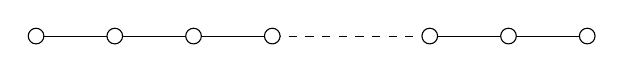
\begin{tikzpicture}
            \draw (0,0) -- (3,0);
            \draw [dashed] (3,0) -- (5,0);
            \draw (5,0) -- (7,0);
            \foreach \x in {0,1,2,3,5,6,7} {
            \node [circle, fill=white, draw=black, inner sep=2pt] at (\x,0) {};
% ---- 原文行 280 ----
            }
        \end{tikzpicture}
    \end{center}
    where vertices represent the spaces $\left(M(X,\phi_i),z_i+z_i^{-1}\right)$ and $P(Y,\xi_i)$, and two vertices are connected by an edge if their representing objects are glued along the fibre/divisor.
\end{crl}
Naturally, we can also connect the first and the last vertices in Corollary \ref{crl:gluing-mirror-symmetry} to obtain mirror symmetries for ``mapping punctured tori'':
\begin{crl}\label{crl:gluing-mirror-symmetry-circ}
    With the same convention as Corollary \ref{crl:gluing-mirror-symmetry}, let \[
        \mathcal{X}_{\circ} (\phi_1,\dotsb,\phi_k)\quad\text{and}\quad\mathcal{Y}_{\circ} (\xi_1,\dotsb,\xi_k)
    \]be Weinstein sectors and algebraic varieties, respectively, obtained by gluing together Weinstein sectors $(M(X,\phi_i),z_i+z_i^{-1})$, resp. $\mathbb{P} (\mathcal{O}_Y\oplus\mathcal{L}_{\xi_i})$ with the same rule as in Corollary \ref{crl:gluing-mirror-symmetry}, with respect to the graph
    \begin{center}
    \begin{tikzpicture}
        % Circle radius
        \def\R{2}
        % Seven vertices equally spaced around the circle
        \coordinate (v1) at (90:\R);
        \coordinate (v2) at (38.571:\R);
        \coordinate (v3) at (-12.857:\R);
        \coordinate (v4) at (-64.286:\R);
        \coordinate (v5) at (-115.714:\R);
% ---- 原文行 300 ----
        \coordinate (v6) at (-167.143:\R);
        \coordinate (v7) at (-218.571:\R);
        % Edges, with the fourth-to-fifth edge dashed
        \draw (v1) arc (90:38.571:\R);
        \draw (v2) arc (38.571:-12.857:\R);
        \draw (v3) arc (-12.857:-64.286:\R);
        \draw (v4) arc (-64.286:-115.714:\R);
        \draw[dashed] (v5) arc (-115.714:-167.143:\R);
        \draw (v6) arc (-167.143:-218.571:\R);
        \draw (v7) arc (-218.571:-270:\R);
        % Vertices
        \foreach \vertex in {v1,v2,v3,v4,v5,v6,v7} {
            \node[circle, fill=white, draw=black, inner sep=2pt]
                at (\vertex) {};
        }
    \end{tikzpicture}
\end{center}
Then we have quasi-equivalences of $A_{\infty}$-categories \[
    \Perf\mathcal{W}\left[\mathcal{X}_{\circ} (\phi_1,\dotsb,\phi_k)\right]^{op}\simeq\Coh\mathcal{Y}_{\circ} (\xi_1,\dotsb,\xi_k)_{dg}.
\]
% ---- 原文行 320 ----
\end{crl}
Together with some deformation argument modified from \cite{LK17}, we should be able to achieve mirror symmetry for fibre bundles with fibres elliptic curves.\par
Aside from gluing pieces together, one can also take direct sums of line bundles on $B$-side and then fibrewise compactify to a toric bundle, while on the $A$-side taking products of $T^{\ast}\mathbb{S}^1$s and putting related stops on the base, using the rules described in \cite{FLTZ12,Kuwagaki20}.\par
More precisely, given mirror pairs $(X;\phi_1,\dotsb ,\phi_k)$ on the $A$-side and $(Y;\xi_1,\dotsb, \xi_k)$ on the $B$-side where $(\phi_1,\dotsb ,\phi_k)$ are mutually commutative symplectomorphisms, together with an integral convex polytope $\Sigma\subseteq\mathbb{R}^k$, one can construct \[
    \mathcal{X}_{\Sigma} (X;\phi_1,\dotsb ,\phi_k )\coloneqq\left(T^{\ast}\mathbb{T}^n,\Lambda_{\Sigma}\right)\times_{\phi_1,\dotsb ,\phi_n} X\to (T^{\ast}\mathbb{T}^n,\Lambda_{\Sigma})
\]as a fibre bundle with fibre $X$ and monodromy around each generator of $\pi_1(\mathbb{T}^n)$ $\phi_i$, and $\mathcal{Y}_{\Sigma} (Y;\xi_1,\dotsb ,\xi_k)$ a fibre bundle over $Y$ with fibres $X_{\Sigma}$, where $(\xi_1,\dotsb ,\xi_k)$ characterizes its structure principal bundle.
\begin{crl}\label{crl:toric-bundle-HMS}
    With the same convention as Corollary \ref{crl:gluing-mirror-symmetry} and let $\Sigma$ be an integral convex polytope in $\mathbb{R}^k$, there is a quasi-equivalence of $A_{\infty}$-categories \[
    \Perf\mathcal{W}\left[\mathcal{X}_{\Sigma} (X;\phi_1,\dotsb ,\phi_k)\right]^{op}\simeq\Coh\left[\mathcal{Y}_{\Sigma} (Y;\xi_1,\dotsb ,\xi_k)\right]_{dg}.
    \]
\end{crl}
\subsection{Hirzebruch surfaces.} As another application, we looked at a particular example of projective toric surfaces that are $\mathbb{P}^1$-bundles over $\mathbb{P}^1$, which are known as \emph{Hirzebruch surfaces}. More precisely, given a non-negative integer $n$, the Hirzebruch surface $\mathbb{F}_n$ is the projectization \[
    \mathbb{F}_n =\mathbb{P}\left(\mathcal{O}_{\mathbb{P}^1}\oplus\mathcal{O}_{\mathbb{P}^1}(n)\right).
\]of the rank $2$ vector bundle $\mathcal{O}\oplus\mathcal{O}_{\mathbb{P}^1} (n)$ over $\mathbb{P}^1$. Since $\mathbb{P}^1$ is toric, $\mathbb{F}_n$ are toric for all $n$.\par
Note that although coherent-constructible correspondence for all toric varieties are known, this result is not compatible with the mirror construction of Hori-Vafa \cite{HV00} when the toric variety is not Fano. For instance, the number of critical points of the Hori-Vafa superpotential $W_n$ is not the same as the rank of the quantum cohomology of the mirror $\mathbb{F}_n$ \cite[Example 8.2]{FOOO10}. The SYZ mirror construction, as explained by Auroux \cite{Auroux09} and later studied by Jing \cite{Jing26}, is highly non-trivial and involves possibly gluing infinitely many charts together.\par
Using theorem \ref{thm:HMS-projective-bundle}, we provide a rather direct description of the homological mirror to $\mathbb{F}_n$.
\begin{crl}\label{crl:mirror-to-Hirzebruch}
    Write \[
        \rF_n =\left(M((\mathbb{C}^{\ast}, x+1/x),\phi^n),z+1/z\right)
    \]to be a Landau-Ginzburg model, where $\phi\colon\mathbb{C}^{\ast}=T^{\ast}\mathbb{S}^1\to T^{\ast}\mathbb{S}^1$ is the Dehn twist along the zero section. Then we have diffeomorphisms as manifolds with boundaries and isomorphisms as holomorphic manifolds with superpotentials\[
% ---- 原文行 340 ----
        \rF_n\cong\left(\mathbb{C}^{\ast}\times\mathbb{C}^{\ast}, x+1/x+y+1/y\right)
    \]and there is a quasi-equivalence of $A_{\infty}$-categories \[
        \Perf\mathcal{W} (\rF_n)^{op}\simeq\Coh\left(\mathbb{F}_n\right)_{dg}.
    \]
\end{crl}
In particular, from the work of Bondal-Orlov \cite{BO01} and Bridgeland-Maciocia \cite{BM01}, we know that $\Coh (\mathbb{F}_n)\cong\Coh (\mathbb{F}_m)$ iff $m=n$, and therefore we immediately get the following possibly interesting Corollary:
\begin{crl}\label{crl:exotic-Weinstein-structure}
    $\rF_n$ is exact symplectomorphic to $\rF_m$ iff $m=n$.
\end{crl}
Therefore although $\rF_n$s are all diffeomorphic and isomorphic as Landau-Ginzburg pairs, they're not exact symplectomorphic and are therefore a sequence of ``exotic'' Weinstein sectors, since exact symplectomorphisms preserve Fukaya categories \cite{HS26}. However, we should note that Fukaya categories cannot distinguish their convex completions and therefore we have no knowledge of whether this creates exotic Weinstein structures on $\left(\mathbb{C}^{\ast}\right)^2$. Another mystery is about the relation between local homological mirror and the Hori-Vafa construction, i.e.
\begin{ques}\label{Q:HV-vs-LHMS}
    What is the relation between the local homological mirror $\rF_n$ and the Hori-Vafa mirror $\left((\mathbb{C}^{\ast})^2,W_n\right)$?
\end{ques}
Answering this question would hopefully provide the desired SYZ mirror for Hirzebruch surfaces via the family Floer program.
\subsection{Structure of the paper.} In section \ref{sec:proof-of-theorems} we provide all the proofs to the statements in the main theorem with technical details postponed to later sections. In section \ref{sec:algebraic-preparations} we give basic definitions of the higher algebras and corresponding operations that we will use throughout the paper. Section \ref{sec:Fukaya-category-discrete-quotient} is devoted to some of the new structural results we need for the $A$-side computation, while sections \ref{sec:G-equiv-sheaves} and \ref{sec:kunneth-formula} establish necessary materials for the $B$-side computation. More explicitly, section \ref{sec:G-equiv-sheaves} provides basic properties of the category of $G$-equivariant sheaves, and section \ref{sec:kunneth-formula} establishes the key formula: the K\"unneth formula for equivariant sheaves. In the appendix \ref{sec:Eilenberg-Zilber-constraction}, we recall the classical Eilenberg-Zilber construction and adapted the construction to our situation, which will be used in the proof of the K\"unneth formula \ref{thm:Kunneth-embedding}.
\subsection*{Acknowledgement.} The main idea of this work arose during the authors' discussion wth Tim Hu and Maximilian Schimpf during their stay in Bonn/Max-Planck-Insititut in late 2025, and we thank all the useful discussions with them.
We also want to thank Yanki Lekili, Cheuk Yu Mak, Longke Tang and Bingyu Zhang for many useful discussions and suggestions.
S.-Y. Liu is funded by the Deutsche Forschungsgemeinschaft (DFG, German Research Foundation) under Germany's Excellence Strategy - GZ 2047/1, Projekt-ID 390685813.
Kyungmin Rho is grateful to Max Planck Institute for Mathematics in Bonn for its hospitality and financial support.
\subsection*{AI disclosure.} The result \cite{BM01} was found with the aid of LLMs when the authors were trying to find the proof that coherent complexes over non-isomorphic Hirzebruch surfaces are not quasi-isomorphic. The authors believed that there should be a better reference than the overly strong result of \cite{BM01}, while the LLM claimed it to be essential.\par
% ---- 原文行 360 ----
The authors used LLMs to explore whether the definition of ``small'' Fukaya category in \ref{defn:wrapped-Fukaya-cat-inf-sectors} is the same as the category of compact objects in $\mathcal{W}^{big} (X)$, without a success. After discussion with Bingyu Zhang and Longke Tang, the authors were convinced that some necessary geometric argument was needed and decided to leave this as a further question to investigate.\par
The reference \cite{Christ26} relating homotopy quotients of an $A_{\infty}$-category $\mathcal{A}$ by a group $G$ to the $A_{\infty}$-orbit category was also found with the aid of LLMs.\par
In the proof of Corollary \ref{crl:gluing-mirror-symmetry}, the authors asked LLM to separate the first huge equation into two rows. The original code was input into LLM and the output was checked and copied directly to the file.\par
The authors tried to find further refernces for the proof of Proposition \ref{prp:dg-enhancement}, and the LLM didn't provide answers outside the authors' knowledge.\par
The authors used LLM to turn the right module action of Seidel \cite{Seidel08} into a left module action, checked and copied the generated codes to the file.
